\section{Mediciones}

Se realizaron mediciones en base a crear pruebas de distintos tamaños y tomar su tiempo de ejecución individualmente, y en base a los datos recolectados hacer el gráfico. Los datos fueron desde 2000 hasta 20.000 elementos, los cuales las ganancias de cada entrenamiento fue generada aleatoriamente entre valores de 1 y 100, y para las energías fueron decayendo en porcentajes. Es decir, el 1\% del total fue 100, otro 99, otro 98... hasta llegar a 1. De esta manera, nos aseguramos de que cada día seguido entrenado cumple con la condición de que la energía de ese día es \textbf{menor o igual} al anterior.

\begin{figure}[H]
	\centering
	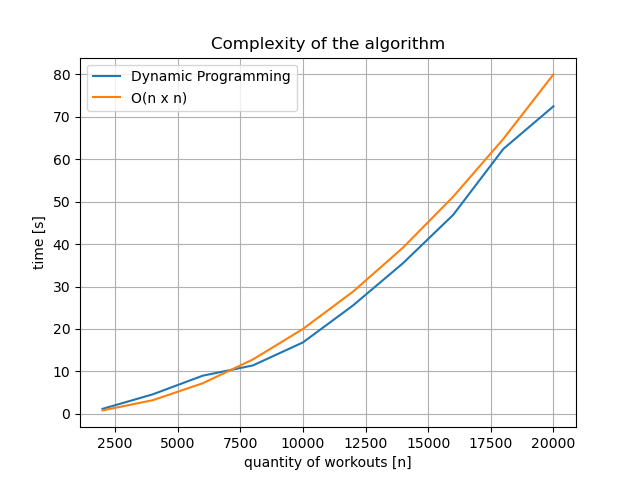
\includegraphics[width=0.9\textwidth]{img/graphic.png}
\end{figure}

Como se puede apreciar, el algoritmo planteado con \textit{Programación Dinámica} efectivamente cumple con la complejidad indicada anteriormente, ya que su diferencia con la complejidad de $\mathcal{O}(n \times n)$ es casi nula\footnote{Aclaracion: para la complejidad indicada por la traza perteneciente a $\mathcal{O}(n \times n)$, se ha dado cierto valor al parámetro $a$ en la ecuación $y=ax^2$ ya que sino para 20.000 elementos el valor $y$ sería igual a 400.000.000, haciendo parecer que nuestro algoritmo es constante.}.
